\documentclass[12pt,a4paper]{article}
\usepackage[utf8]{inputenc}
\usepackage[T1]{fontenc}
\usepackage{amsmath}
\usepackage{amsfonts}
\usepackage[francais]{babel}
\usepackage{amssymb}
\usepackage{graphicx}
\usepackage[top=2.00cm]{geometry}
\usepackage{enumitem}
%\usepackage{tikz}
%\usepackage{mathtools}
%\usepackage{pgfplots}
%\usetikzlibrary{plotmarks}
\usepackage{bigcenter}
\usepackage{multicol}

%Modif des enumerates numeros en gras. leftmargin=*,
\setlist[enumerate]{label=\textbf{\arabic*}.}

\usepackage{titlesec}
%modif des titres de section diminuer la taille
\titleformat{\section}
  {\normalfont\fontsize{14}{15}\bfseries}{\thesection}{1em}{}
\titleformat{\subsection}
  {\normalfont\fontsize{12}{15}\bfseries}{\thesubsection}{1em}{}


\author{CHARNAIS Valentin, FINOT Sylvain}
\title{Compte rendu de TP : \\ Régulation de tension}

\begin{document}
\maketitle
L'objectif de ce TP est de comparer différents montages permettant d'obtenir une tension continue a partir d'alternatif.
\section{Redressement et filtrage}
%\subsection{Étude du montage à basse fréquence (Amplificateur Opérationnel considéré idéal)}
\begin{enumerate}
\item Nous cherchons a obtenir un signal continu a partir d'un générateur de tension alternatif 7V. Pour ce faire nous utilisons un pont de diodes (pont de Graëtz) qui permet dans un premier temps de redresser la partie négative du signal. Le signal ressemble alors à la valeur absolue d'une sinusoïde. Cependant nous cherchons a obtenir un signal continu. Il suffit alors de mettre un condensateur en parallèle, celui ci va jouer le rôle de réservoir ("buffer"), permettant ainsi d'obtenir un signal relativement continu/stable. Cela veut donc dire que ce montage marche bien lorsque l'utilisateur ne demande pas trop de courant et donc que la décharge du condensateur est minime $\implies$ $R_{c}$ très grand.\\
Une fois le montage réalisé, on peut être tenté de regarder simultanément sur l'oscilloscope le signal en sortie du générateur et le signal au bornes du condensateur. C'est une très mauvaise idée, cela reviendrait a court-circuiter une des diodes du pont puisque deux de ses bornes seraient reliés au même point, la masse de l'oscilloscope.

\item On observe par la suite la différence entre le signal de sortie avec R$_{c}$=1k$\Omega$ et sans R$_{c}$ $\iff$ R$_{c}=+ \infty$. On remarque que le taux d'ondulation : \[T\equiv \dfrac{\delta V}{V} \] est beaucoup plus important lorsque R$_{c}=1$k$\Omega$. \\
On essaye alors de mesurer T avec précision, on regarde d'abord la tension de sortie puis uniquement le taux d'ondulation.
\begin{multicols}{2}
\begin{itemize}
\item Pour R$_{c}=+ \infty$ :\\
% Pas sur du calibre pour T
U$_{s}=10$V \\
T=0,2mV (calibre 1mV/div)
\item Pour R$_{c}$=1k$\Omega$ : \\
U$_{s}=9$V\\
T=80mV (calibre 20mV/div)
\end{itemize}
\end{multicols}
\end{enumerate}
Dans ce TP nous cherchons à mesurer les performances de différents montages permettant d'avoir une tension continue. Nous allons pour cela faire varier R$_{c}$ pour simuler différents appareils. Nous devons cependant veiller a ne pas dépasser 0,25W par résistance. Il va donc falloir mettre des résistances en parallèles pour atteindre des faibles valeurs de R$_{c}$ sans dépasser 0,25W.
%\begin{multicols}{2}
\\Nous utilisons un générateur alternatif de 7V, la tension efficace est donc U$_{eff}$=$\sqrt{2}$U$\approx$10V\\
\begin{align*}
P=\dfrac{U^{2}}{R}&<0,25\\
\implies R&>\dfrac{U^{2}}{0,25}=400\Omega
\end{align*}
%\end{multicols}
\textbf{A COMPLÉTER}
\begin{enumerate}
\item On remarque que le taux d'ondulation se dégrade lorsque R$_{c}$ diminue. En effet, pour de faibles valeurs de R$_{c}$ le courant appelé est élevé, le condensateur se décharge grandement et n'arrive plus a suivre si sa capacité est trop faible. Nous pensons que le condensateur se charge pendant la phase croissante de tension, puis se décharge lorsque l'alimentation ne fournit plus assez. Il agit comme un accumulateur.
\begin{multicols}{2}
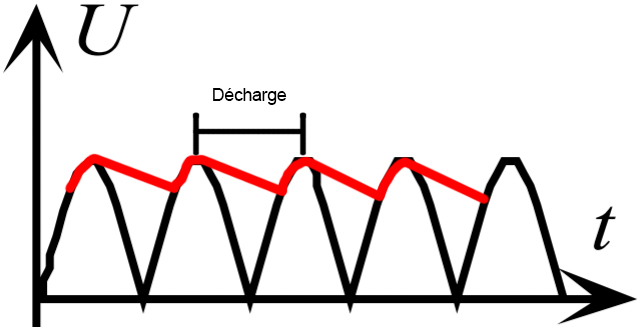
\includegraphics[scale=0.25]{Condensateur}
\columnbreak
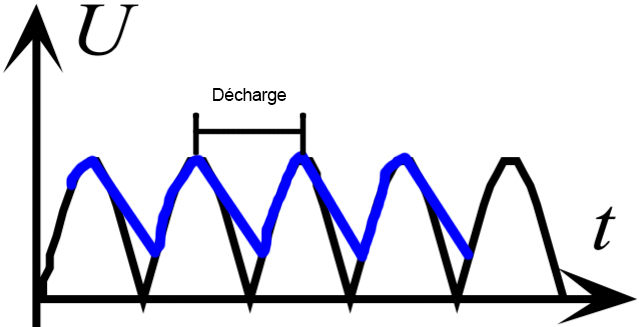
\includegraphics[scale=0.25]{Condensateur2}
\end{multicols}
A droite le courant appelé est plus important qu'a gauche, la régulation est moins bonne.
\item en prenant un condensateur de 10$\mu$F, on remarque de la sortie est beaucoup moins stable (V$\in$[1V;10V]) qu'avec le condensateur de 1000$\mu$F que nous utilisons. Notre interprétation semble être correcte.
\end{enumerate}
\section{RÉGULATION PAR DIODE ZENER SIMPLE}
Nous allons à présent tenter d'améliorer la régulation en ajoutant une diode Zener et une résistance à la suite du montage précédent.
\begin{figure}[h]
\centering
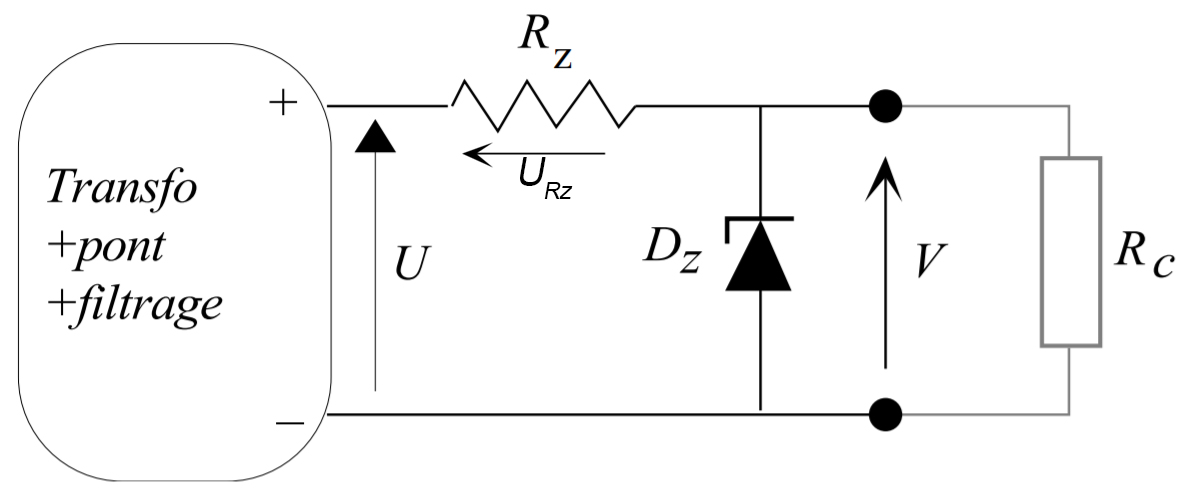
\includegraphics[scale=0.25]{Zener}
\caption[Montage avec diode Zener]{Montage avec diode Zener}
\label{fig:zener}
\end{figure}
Avant toute chose, nous devons faire attention à ne pas dissiper plus de 0,5W dans la diode Zener et plus de 0,25W dans la résistance R$_{z}$. On étudie le cas limite, i.e R$_{c}$=$\infty$, tout le courant va dans la Diode.
%\begin{multicols}{2}
\[
\begin{aligned}
\begin{cases}
P_{z}=V.I_{tot}\\
R_{z}=\dfrac{(U-V)}{I_{tot}}
\end{cases}
\end{aligned}
\iff
\begin{aligned}
\begin{cases}
I_{tot}=\dfrac{P_{z}}{V}\\
R_{z}=\dfrac{(U-V)V}{P_{z}}
\end{cases}
\implies R_{z}=\dfrac{(10-8,2)8,2}{0,5}=30\Omega
\end{aligned}
\]
Il faut donc R$_{z}$>30$\Omega$ pour ne pas dissiper plus de 0,5W dans la diode Zener, mais comment faut-il choisir R$_{z}$ pour qu'elle ne grille pas (P$_{R_{z}}$<0,25W)

\begin{align*}
P_{R_{z}}&<0,25W\\ \iff \dfrac{(U_{z})^{2}}{R_{z}}&<0,25W \iff \dfrac{(U-V)^{2}}{R_{z}}<0,25W\\
\iff R_{z}&>4.(U-V)^{2}\\
\implies R_{z}&>4.(10-8,2)^{2}=13\Omega
\end{align*}
Il faut que : 
\[
\begin{cases}
R_{z}>30\Omega\\
R_{z}>13\Omega
\end{cases}
\implies R_{z}>30\Omega
\]
Dans notre cas nous resterons largement au dessus de 30$\Omega$

\end{document}
